\phantomsection
\section*{Глава 3. Разработка веб-приложения}
\addcontentsline{toc}{section}{Глава 3. Разработка веб-приложения}
\stepcounter{section}

\subsection{Структура программной части проекта}

Разработка веб-приложения выполнена с использованием фреймворка Django. Проект состоит из основного Django-проекта, приложения предметной области, HTML-шаблонов, статических файлов и каталога для пользовательских медиафайлов.

Основная программная часть расположена в каталоге \texttt{app}. Внутри него находятся файл управления проектом \texttt{manage.py}, каталог настроек \texttt{library\_project}, приложение \texttt{library}, виртуальное окружение разработки и каталог \texttt{media} для загружаемых файлов.

Структура основных файлов программной части представлена в таблице~\ref{tab:project-structure}.

\begin{table}[htbp]
\centering
\caption{Структура программной части проекта}
\label{tab:project-structure}
\small
\begin{tabular}{|p{0.34\textwidth}|p{0.56\textwidth}|}
\hline
\textbf{Файл или папка} & \textbf{Назначение} \\
\hline
\texttt{manage.py} &
Управляющий файл Django-проекта, используемый для запуска сервера, выполнения миграций и административных команд. \\
\hline
\texttt{library\_project/settings.py} &
Файл настроек проекта: подключение приложений, настройка базы данных, статических и медиафайлов, чтение переменных окружения. \\
\hline
\texttt{library\_project/urls.py} &
Корневой файл маршрутизации проекта, подключающий маршруты приложения \texttt{library} и административную панель Django. \\
\hline
\texttt{library/models.py} &
Описание моделей данных предметной области: книг, авторов, категорий, читателей и выдач. \\
\hline
\texttt{library/forms.py} &
Описание форм регистрации, добавления и редактирования книг, оформления выдачи и редактирования читателя. \\
\hline
\texttt{library/views.py} &
Реализация функций обработки запросов, бизнес-логики приложения, фильтрации, сортировки, статистики и выгрузки CSV. \\
\hline
\texttt{library/urls.py} &
Маршруты приложения: главная страница, каталог, карточка книги, журнал выдач, статистика, авторизация, регистрация и управление читателями. \\
\hline
\texttt{library/templates/} &
HTML-шаблоны страниц пользовательского интерфейса. \\
\hline
\texttt{library/static/} &
Статические файлы приложения, в том числе пользовательские стили CSS. \\
\hline
\texttt{media/covers/} &
Локальный каталог для загруженных пользователем обложек книг. \\
\hline
\end{tabular}
\end{table}

Главная страница приложения содержит краткое описание назначения системы и основные переходы к разделам приложения. Вид главной страницы представлен на рисунке~\ref{fig:app-home}.

\begin{figure}[htbp]
\centering
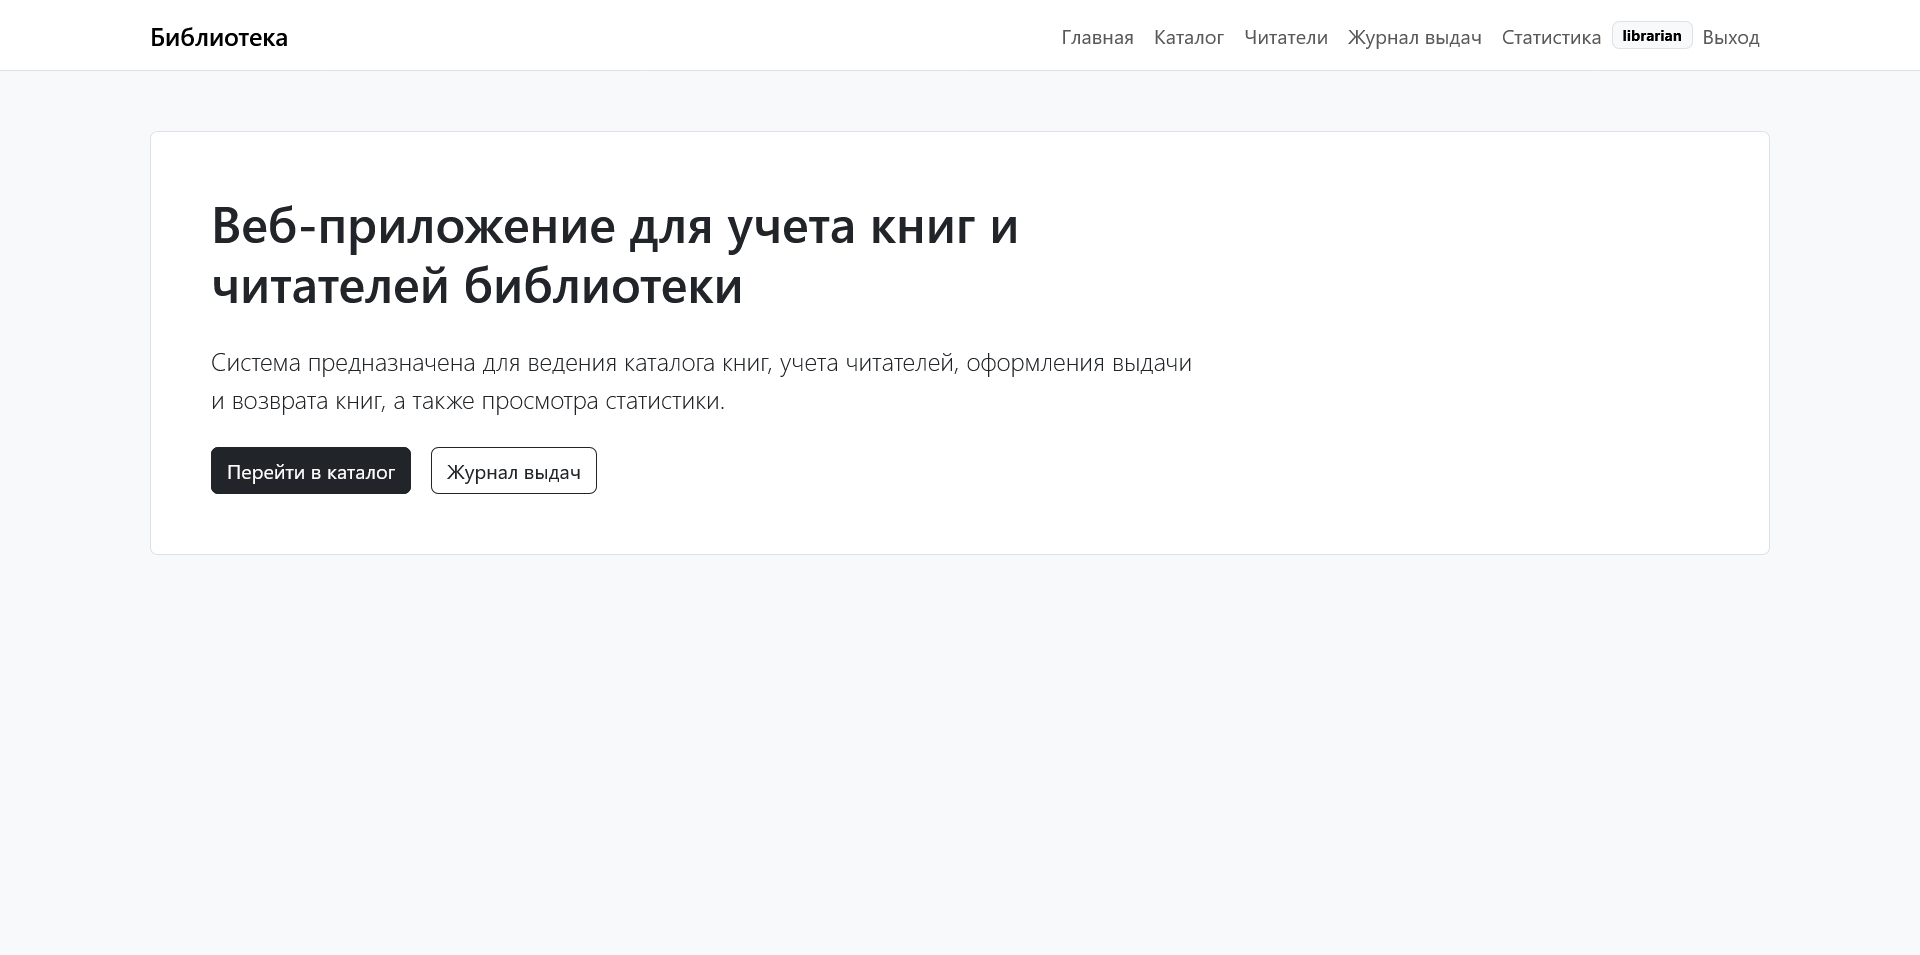
\includegraphics[width=0.90\textwidth]{images/app_home.png}
\caption{Главная страница веб-приложения}
\label{fig:app-home}
\end{figure}

\subsection{Настройка проекта и базы данных}

В качестве базы данных используется SQLite. Данный вариант подходит для учебного проекта, так как не требует отдельной установки сервера базы данных и позволяет быстро развернуть приложение на локальном компьютере.

В файле \texttt{settings.py} подключены стандартные приложения Django, приложение \texttt{library}, настройки шаблонов, статических файлов и медиафайлов. Загружаемые обложки книг сохраняются в каталоге \texttt{media/covers/}, а путь к файлу хранится в поле \texttt{cover} модели \texttt{Book}.

Для повышения безопасности секретный ключ Django вынесен в переменные окружения и считывается из файла \texttt{.env}. В репозиторий файл \texttt{.env} не добавляется, так как он содержит локальные настройки проекта.

\subsection{Реализация моделей данных}

Модели данных реализованы в файле \texttt{library/models.py}. Основными сущностями приложения являются:

\begin{itemize}
    \item \texttt{Reader} --- читатель библиотеки;
    \item \texttt{Author} --- автор книги или авторский коллектив;
    \item \texttt{Category} --- категория книги;
    \item \texttt{Book} --- конкретное издание книги;
    \item \texttt{BookAuthor} --- промежуточная сущность связи книги и автора;
    \item \texttt{BookCategory} --- промежуточная сущность связи книги и категории;
    \item \texttt{Loan} --- запись о выдаче книги читателю.
\end{itemize}

Модель \texttt{Book} содержит название, год издания, состав томов, описание, количество экземпляров, количество доступных экземпляров и поле для обложки. Авторы и категории связаны с книгами отношениями многие-ко-многим через промежуточные модели. Такой подход позволяет указывать для одной книги нескольких авторов и несколько категорий.

Для модели \texttt{Reader} реализовано хранение ФИО, телефона, даты регистрации и связи с учетной записью пользователя Django. Телефон нормализуется при сохранении и приводится к единому формату.

Модель \texttt{Loan} хранит данные о выдаче: книгу, читателя, дату выдачи, срок возврата, фактическую дату возврата и статус. Для статуса используются значения «выдана», «возвращена» и «просрочена».

\subsection{Реализация авторизации и разграничения прав}

Для авторизации используется встроенная система пользователей Django. В приложении предусмотрены три роли:

\begin{itemize}
    \item читатель;
    \item библиотекарь;
    \item администратор.
\end{itemize}

Читатель может просматривать каталог и карточки книг. Библиотекарь имеет доступ к управлению каталогом, читателями, выдачами, статистикой и CSV-выгрузкам. Администратор управляет пользователями и группами через административную панель Django.

Форма входа в систему представлена на рисунке~\ref{fig:app-login}.

\begin{figure}[htbp]
\centering
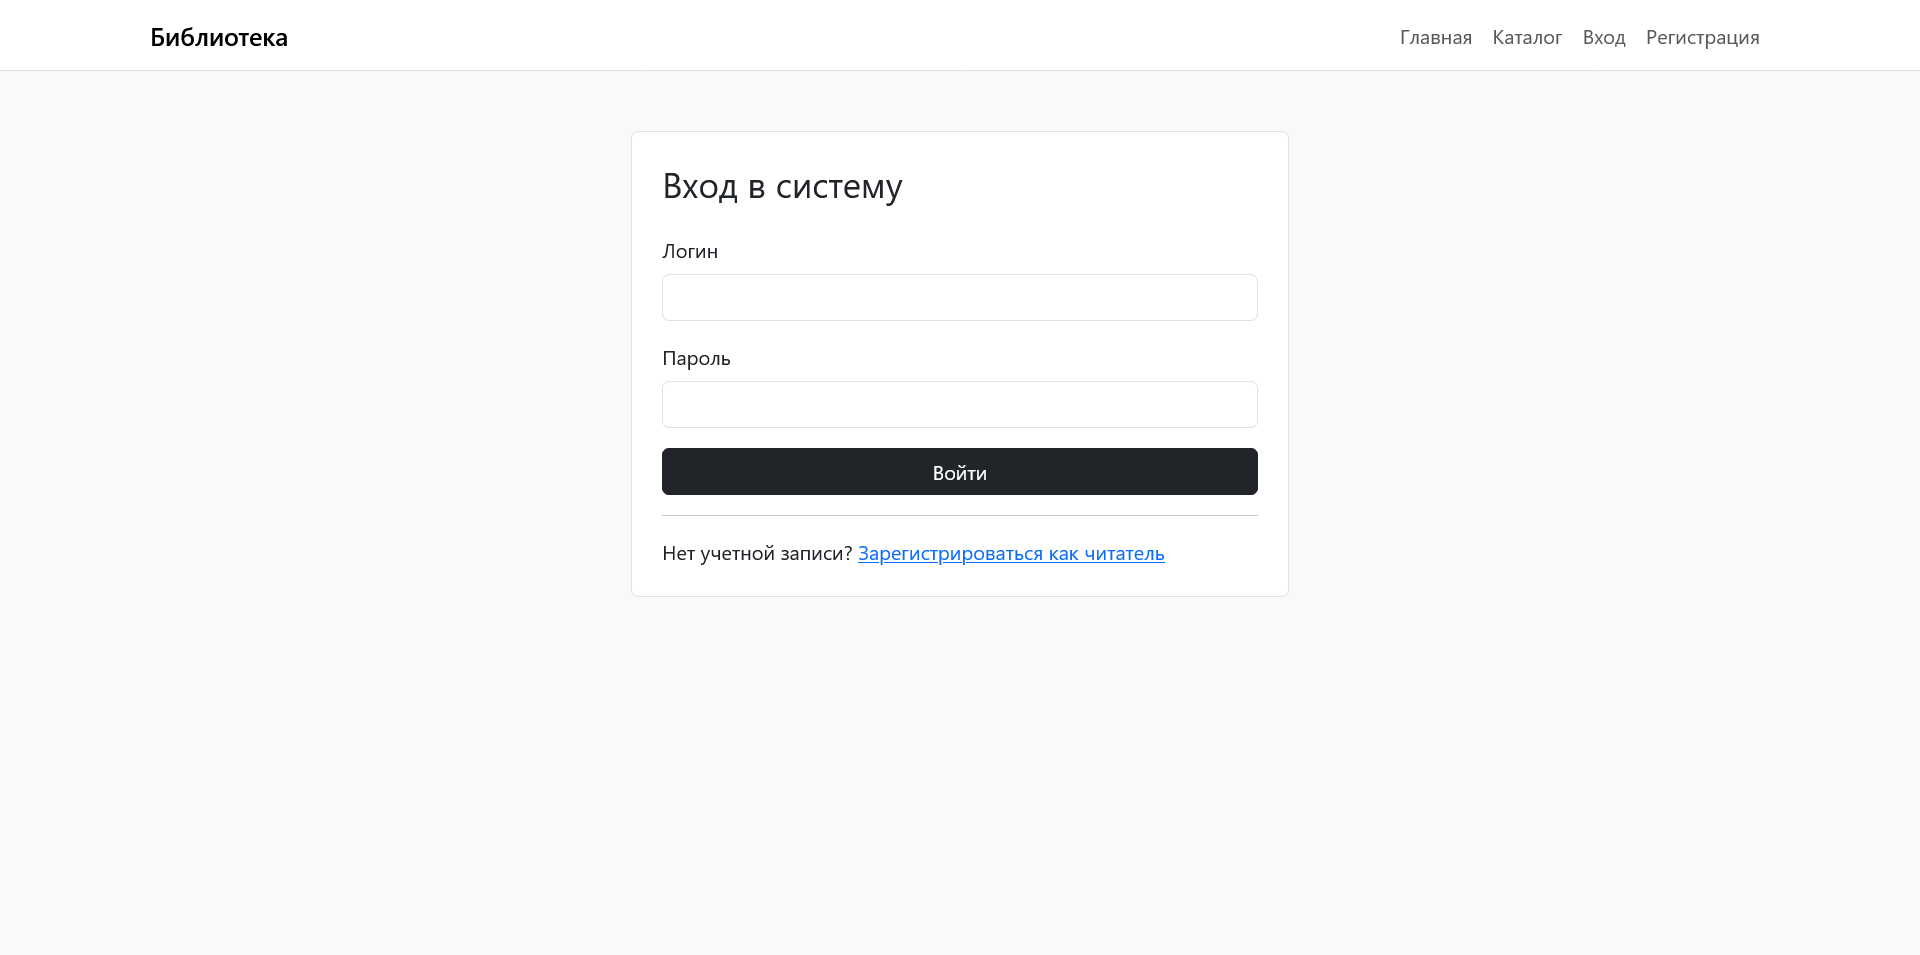
\includegraphics[width=0.80\textwidth]{images/app_login.png}
\caption{Страница авторизации пользователя}
\label{fig:app-login}
\end{figure}

Административная панель Django используется для управления учетными записями, группами и справочными данными. Вид административной панели представлен на рисунке~\ref{fig:app-admin}.

\begin{figure}[htbp]
\centering
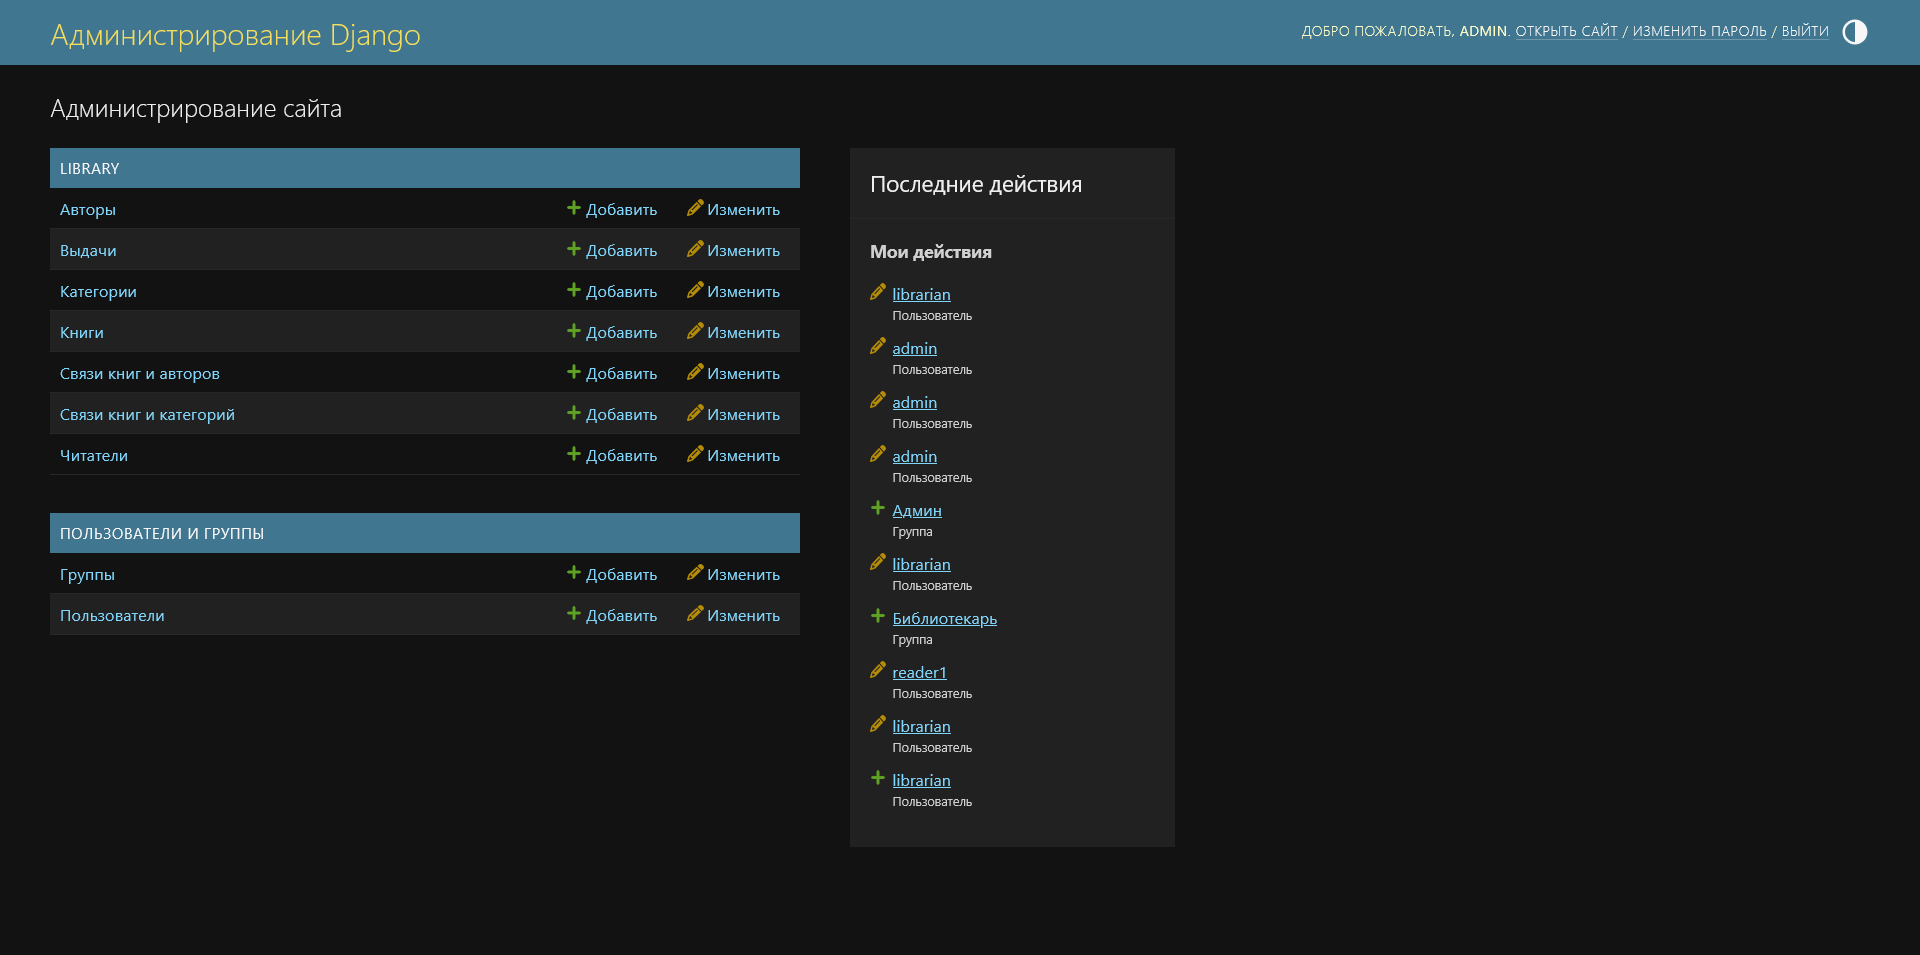
\includegraphics[width=0.90\textwidth]{images/app_admin.png}
\caption{Административная панель Django}
\label{fig:app-admin}
\end{figure}

Разграничение доступа реализовано на уровне представлений. Перед выполнением действий, доступных только библиотекарю, проверяется принадлежность пользователя к группе \texttt{Библиотекарь}. Если пользователь не имеет нужной роли, он перенаправляется в каталог.

\subsection{Реализация каталога книг}

Каталог книг является основным разделом приложения. Он отображает список книг, обложки, авторов, категории, количество изданий и доступность экземпляров. Для удобства пользователя реализованы поиск, фильтрация и сортировка.

В каталоге доступны следующие возможности:

\begin{itemize}
    \item поиск по названию книги;
    \item фильтрация по автору;
    \item фильтрация по категории;
    \item фильтрация по наличию доступных экземпляров;
    \item сортировка по названию, авторам, категориям, числу изданий и доступности;
    \item раскрытие списка изданий одной книги;
    \item переход в карточку книги;
    \item выгрузка каталога в CSV.
\end{itemize}

Страница каталога книг представлена на рисунке~\ref{fig:app-catalog}.

\begin{figure}[htbp]
\centering
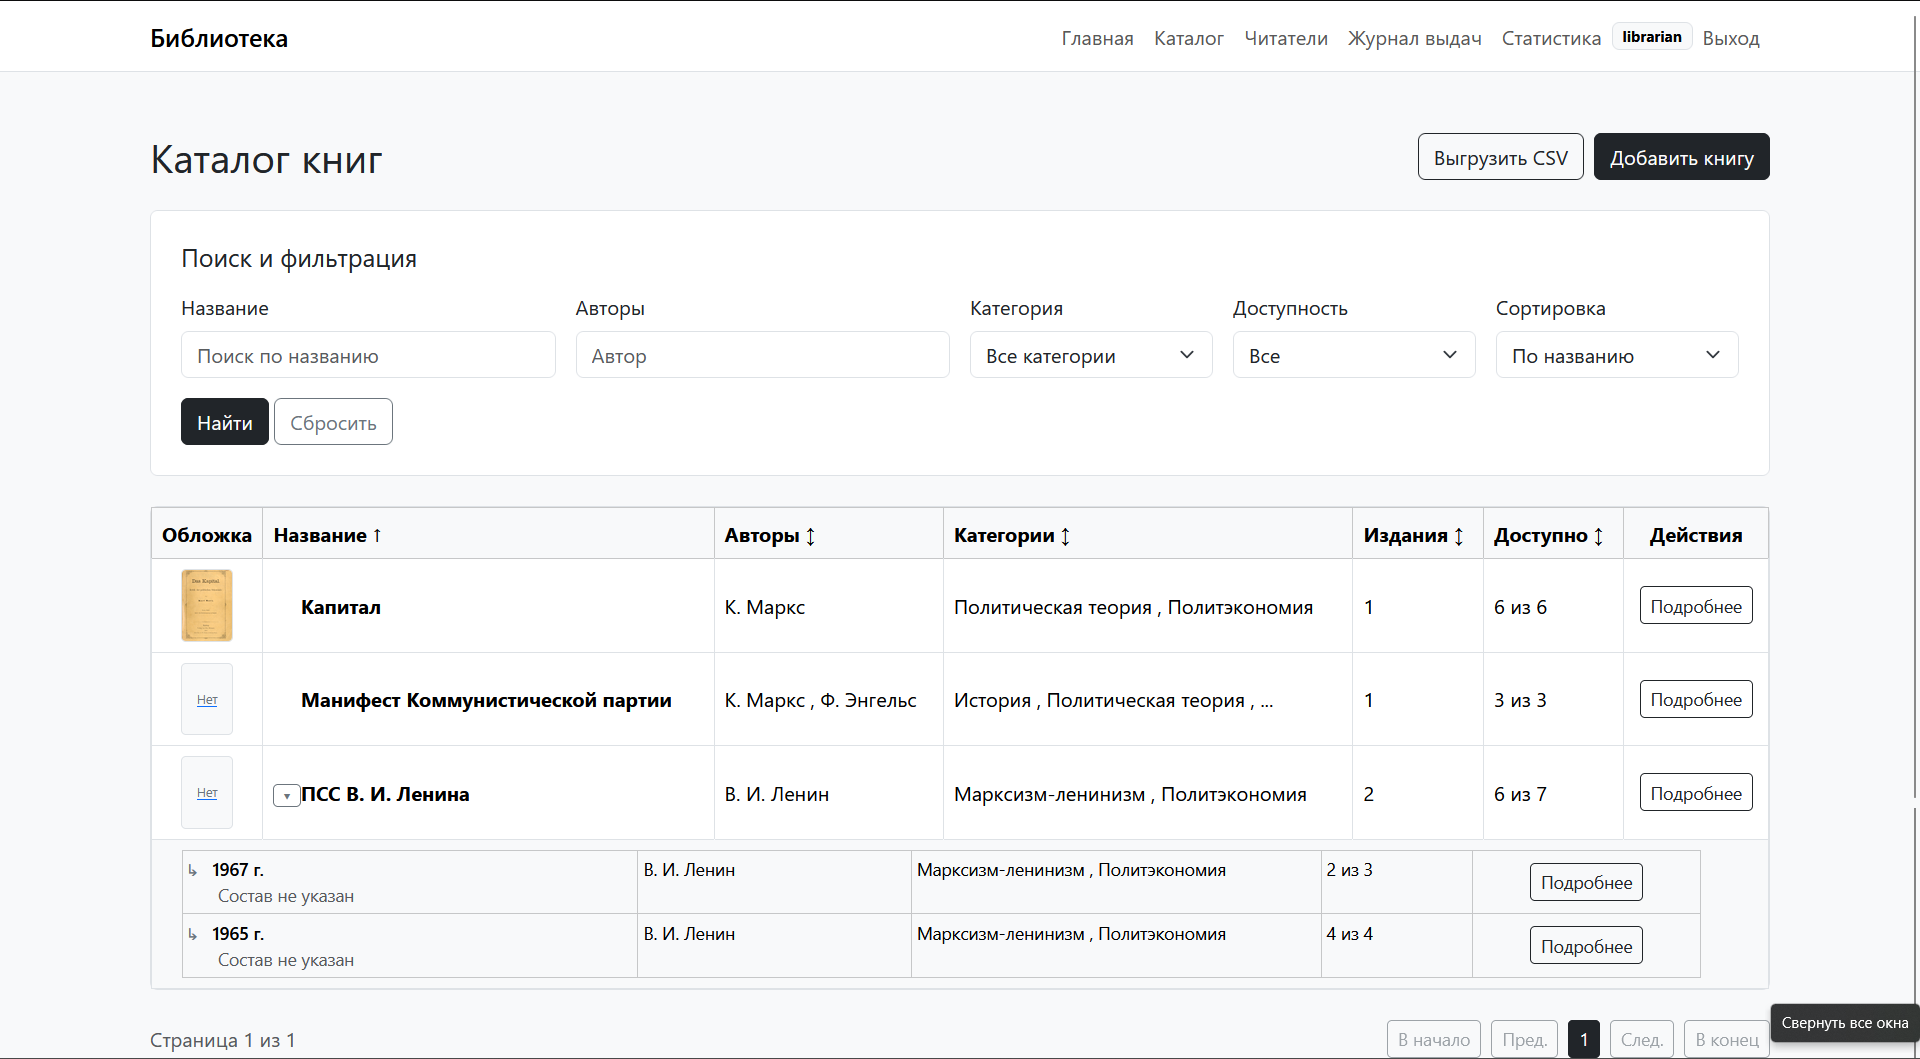
\includegraphics[width=0.95\textwidth]{images/app_catalog.png}
\caption{Каталог книг с поиском, фильтрацией, сортировкой и раскрытием изданий}
\label{fig:app-catalog}
\end{figure}

Разные издания одной книги группируются по названию и составу авторов. Основной строкой показывается сводная информация, а вложенные строки отображают конкретные издания с годом издания, составом томов и доступностью.

\subsection{Реализация карточки книги}

Карточка книги содержит подробную информацию о конкретном издании: название, авторов, год издания, состав томов, категории, доступность, описание и обложку. Для библиотекаря на странице доступны действия оформления выдачи, редактирования и удаления книги.

Карточка книги представлена на рисунке~\ref{fig:app-book-detail}.

\begin{figure}[htbp]
\centering
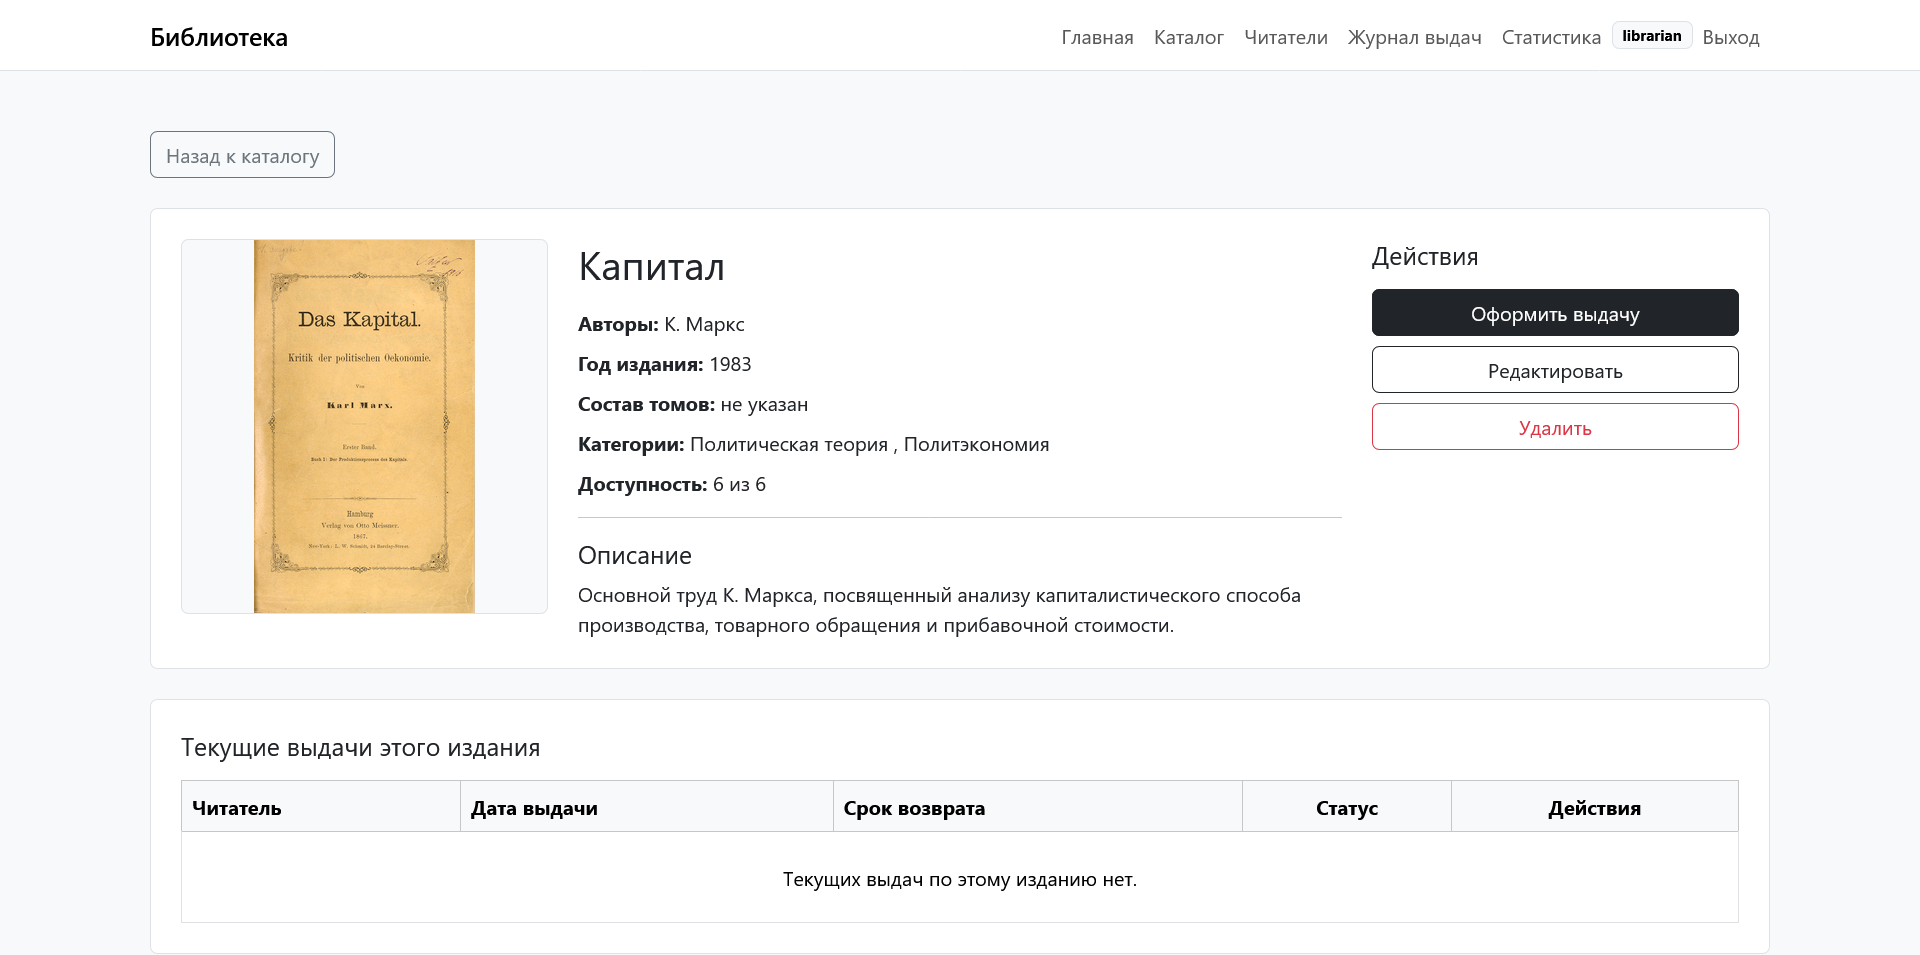
\includegraphics[width=0.95\textwidth]{images/app_book_detail.png}
\caption{Карточка книги}
\label{fig:app-book-detail}
\end{figure}

Если у книги есть текущие выдачи, библиотекарь видит их в отдельной таблице на странице карточки. Это позволяет быстро определить, у каких читателей находится выбранное издание.

Форма добавления и редактирования книги включает поля названия, авторов, категорий, года издания, состава томов, количества экземпляров, описания и обложки. Вид формы редактирования книги представлен на рисунке~\ref{fig:app-book-form}.

\begin{figure}[htbp]
\centering
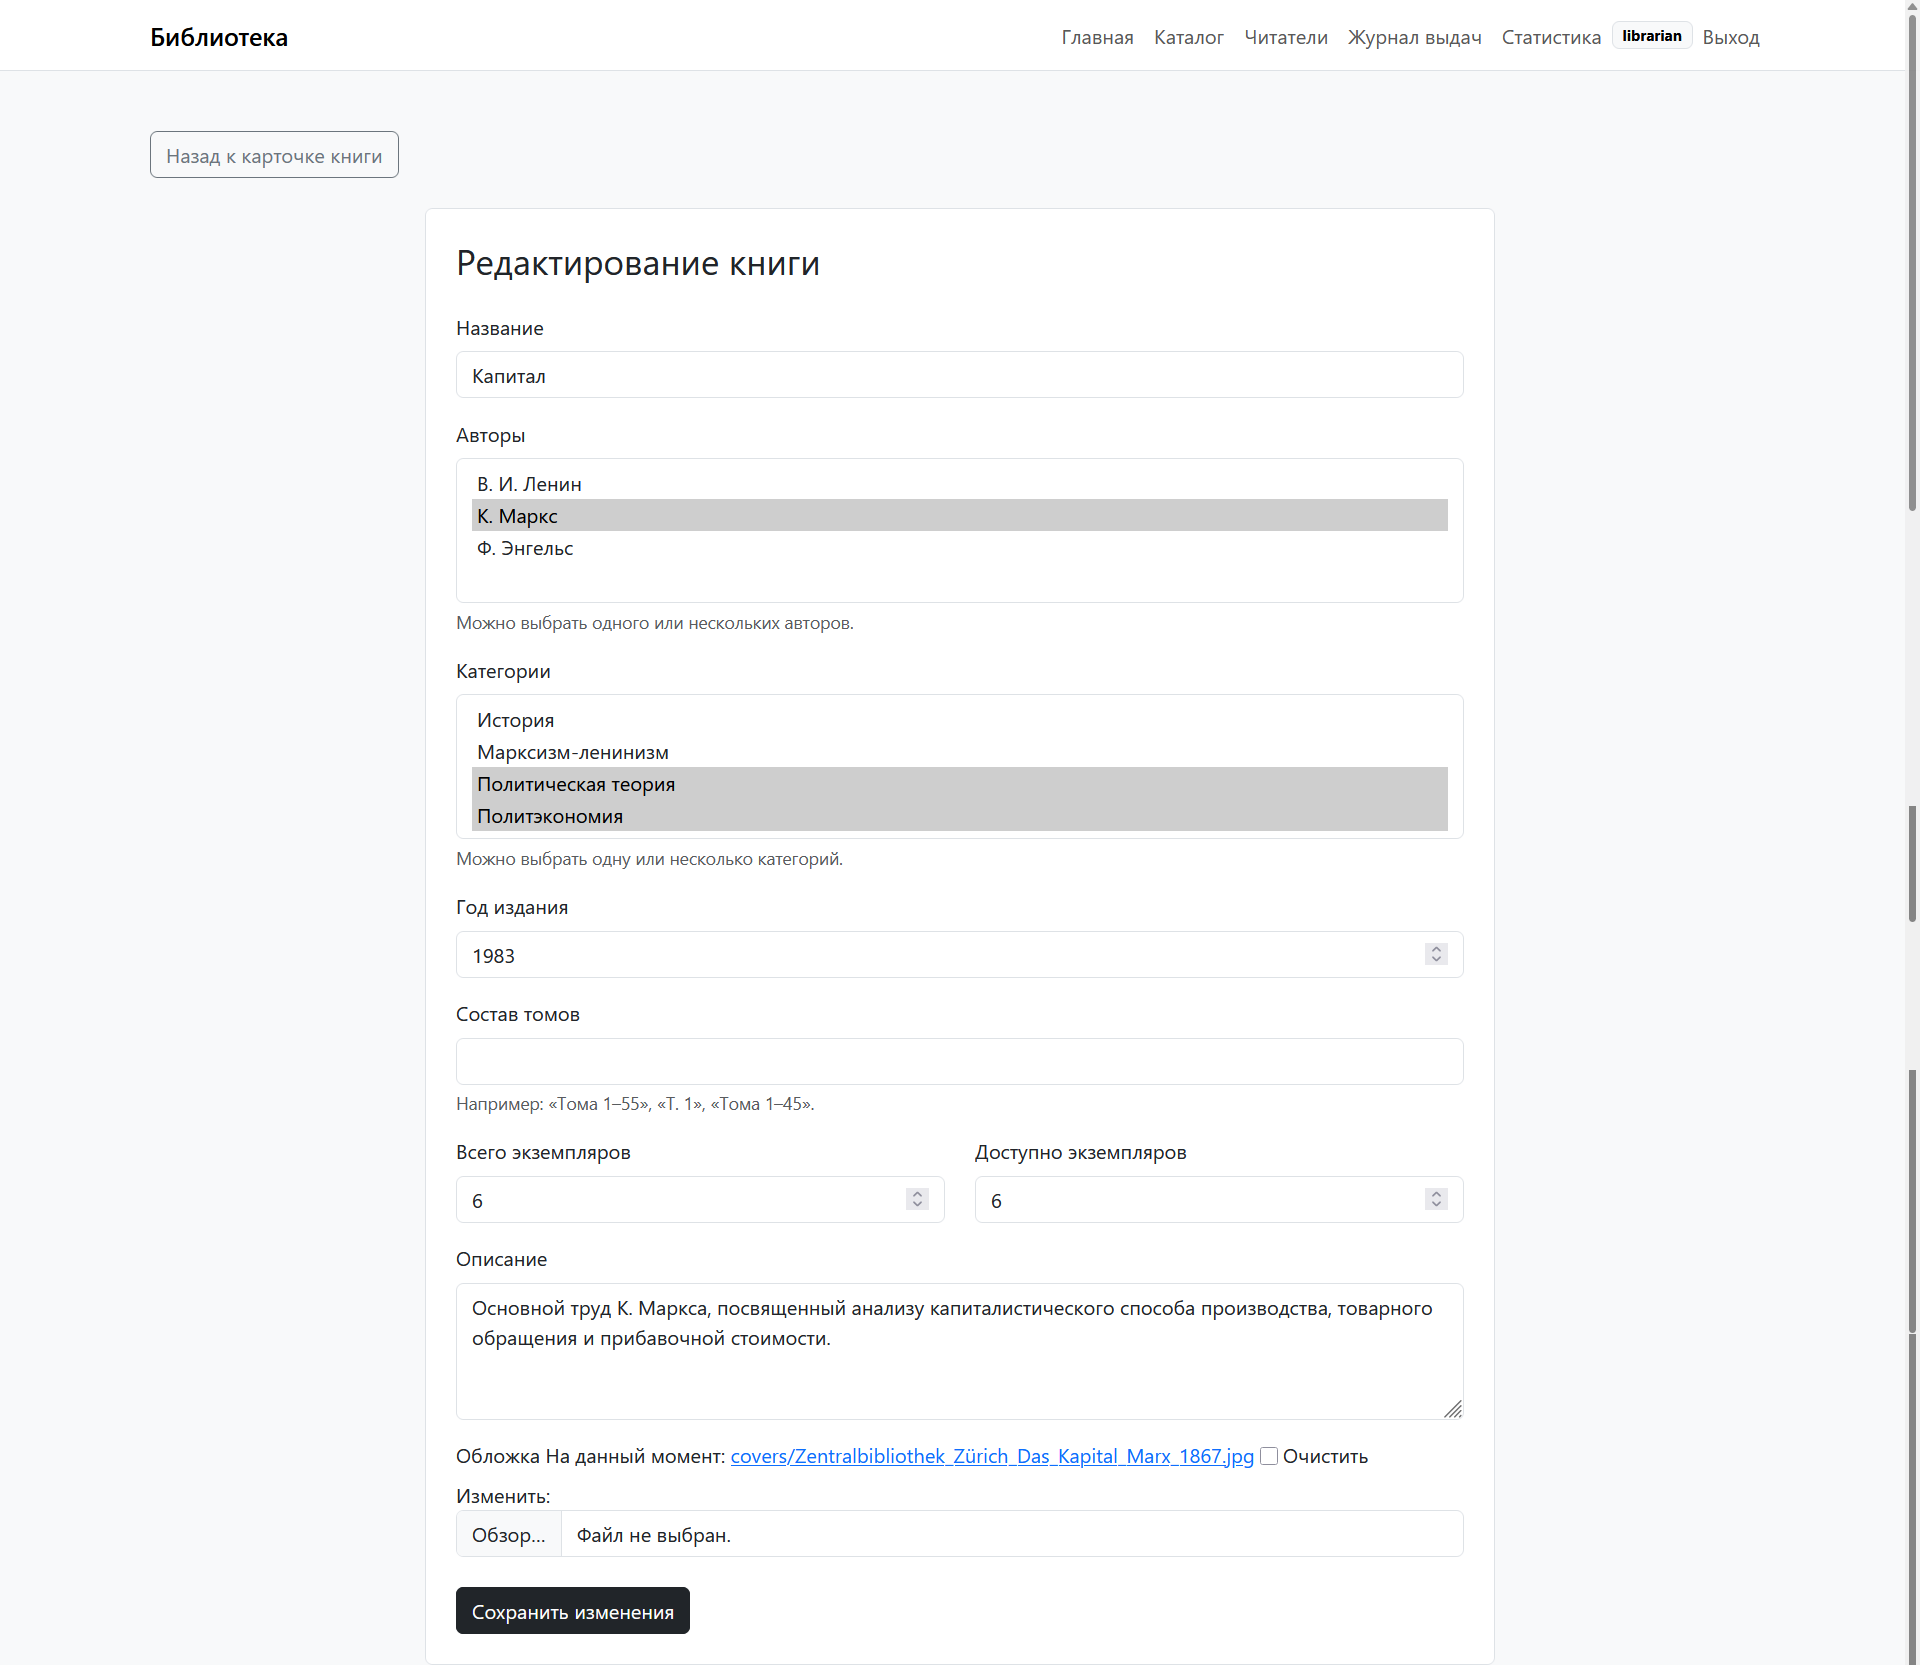
\includegraphics[width=0.85\textwidth]{images/app_book_form.png}
\caption{Форма добавления и редактирования книги}
\label{fig:app-book-form}
\end{figure}

При сохранении книги проверяется корректность количества экземпляров: число доступных экземпляров не может быть больше общего количества.

\subsection{Реализация учета читателей}

Для работы с читателями реализован отдельный раздел. Библиотекарь может просматривать список читателей, искать читателя по ФИО, телефону, электронной почте или логину, а также переходить в карточку читателя.

Страница списка читателей представлена на рисунке~\ref{fig:app-readers}.

\begin{figure}[htbp]
\centering
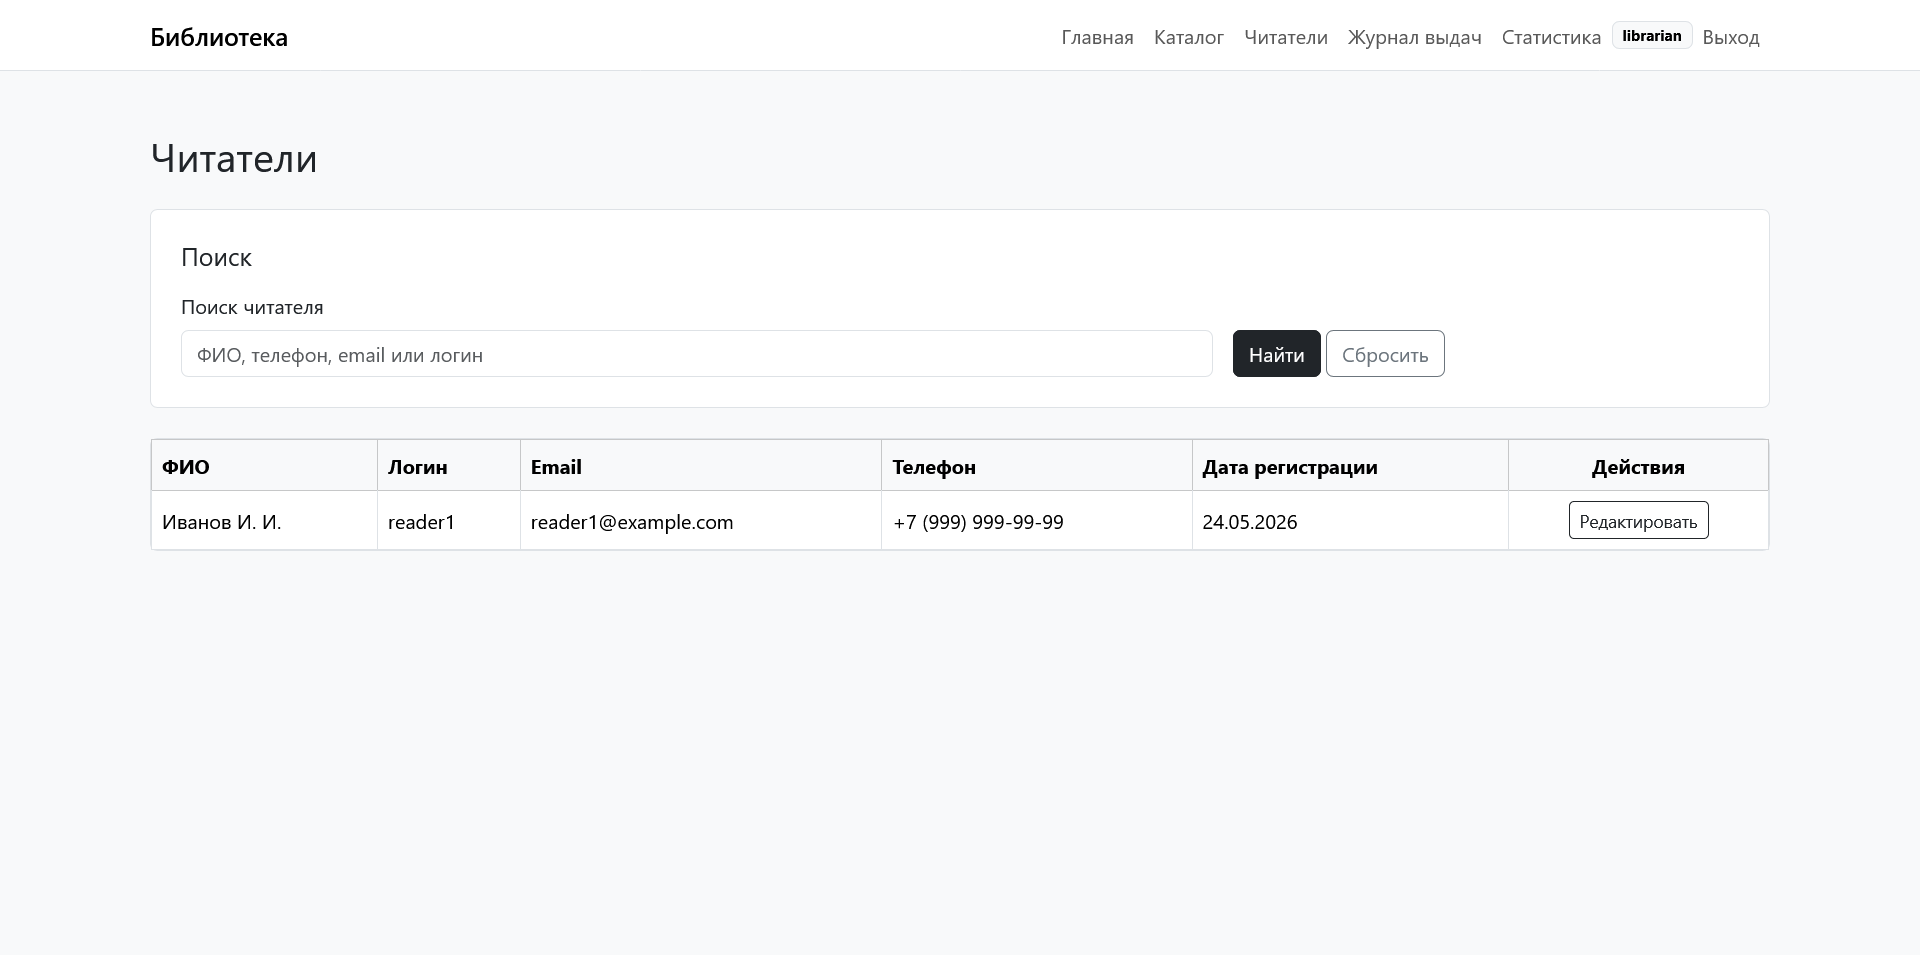
\includegraphics[width=0.95\textwidth]{images/app_readers.png}
\caption{Список читателей}
\label{fig:app-readers}
\end{figure}

Карточка читателя содержит логин, электронную почту, телефон, дату регистрации и историю выдач. Вид карточки читателя представлен на рисунке~\ref{fig:app-reader-detail}.

\begin{figure}[htbp]
\centering
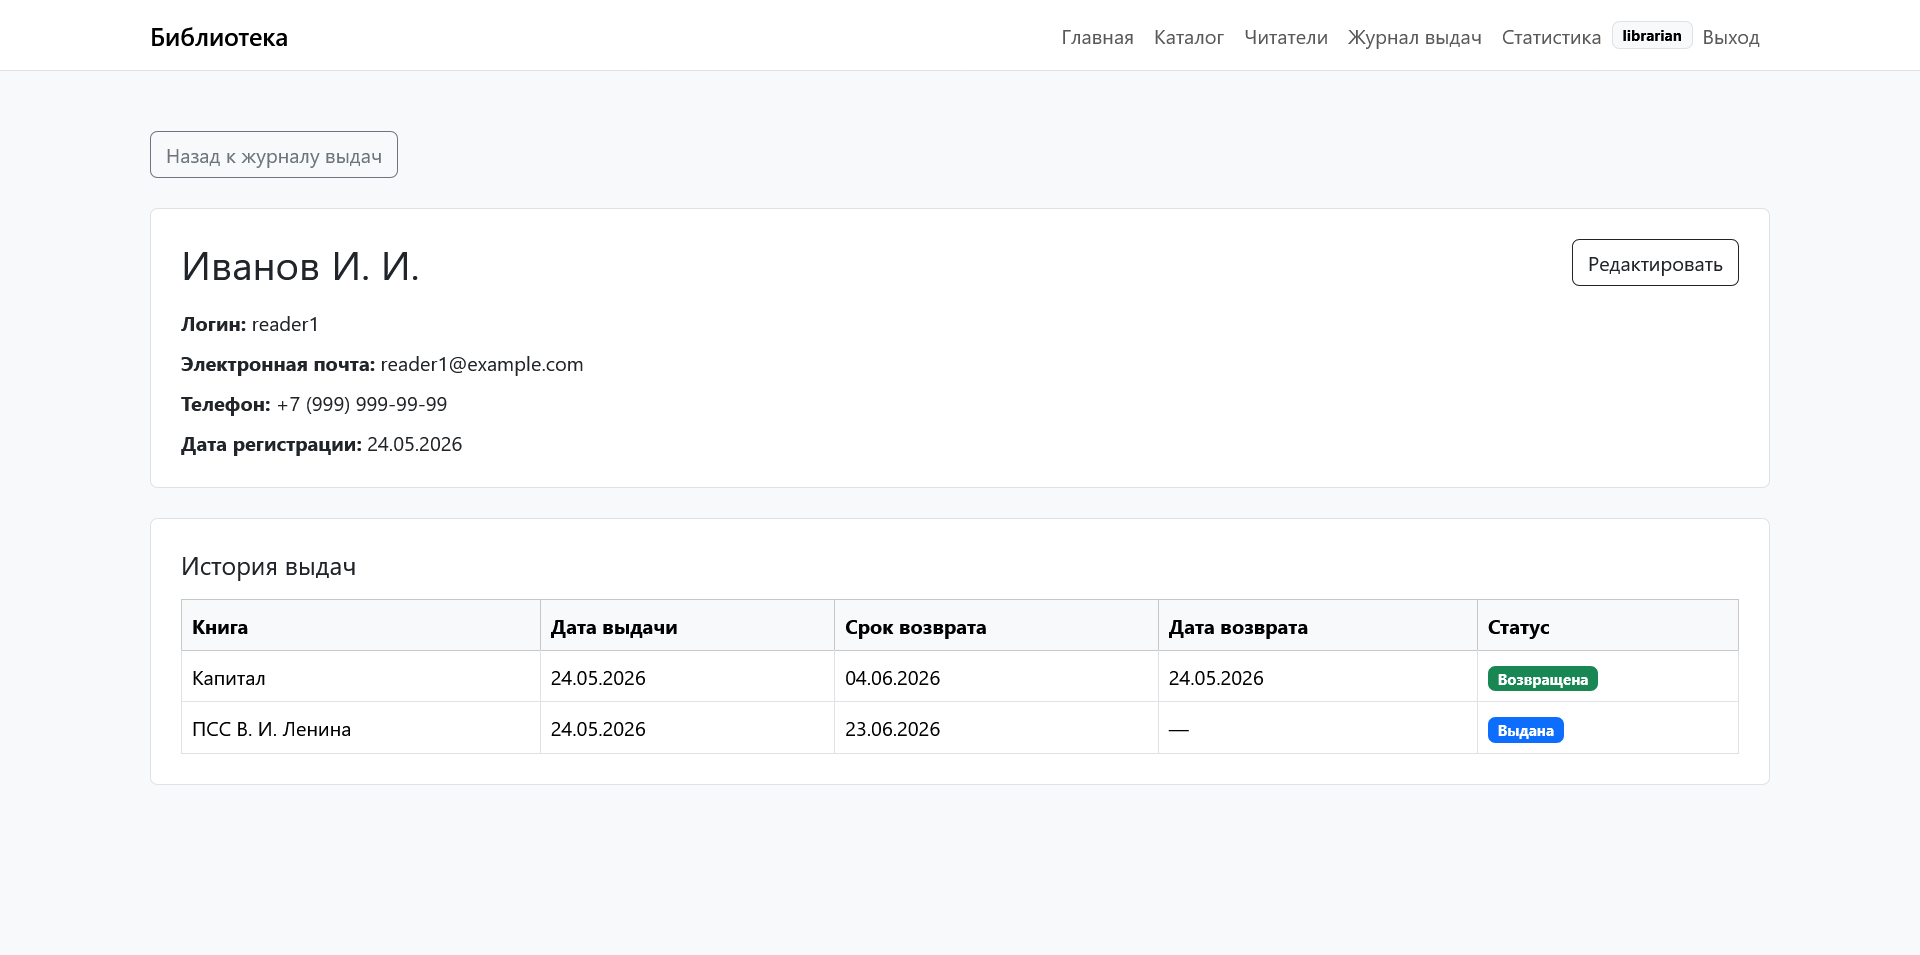
\includegraphics[width=0.95\textwidth]{images/app_reader_detail.png}
\caption{Карточка читателя с историей выдач}
\label{fig:app-reader-detail}
\end{figure}

История выдач показывает, какие книги были выданы читателю, когда они были выданы, какой установлен срок возврата, была ли книга возвращена и какой статус имеет выдача.

\subsection{Реализация оформления и возврата книг}

Оформление выдачи доступно библиотекарю. При оформлении выбираются книга, читатель, дата выдачи и срок возврата. По умолчанию дата выдачи устанавливается равной текущей дате, а срок возврата --- на один месяц позже.

Форма оформления выдачи представлена на рисунке~\ref{fig:app-loan-form}.

\begin{figure}[htbp]
\centering
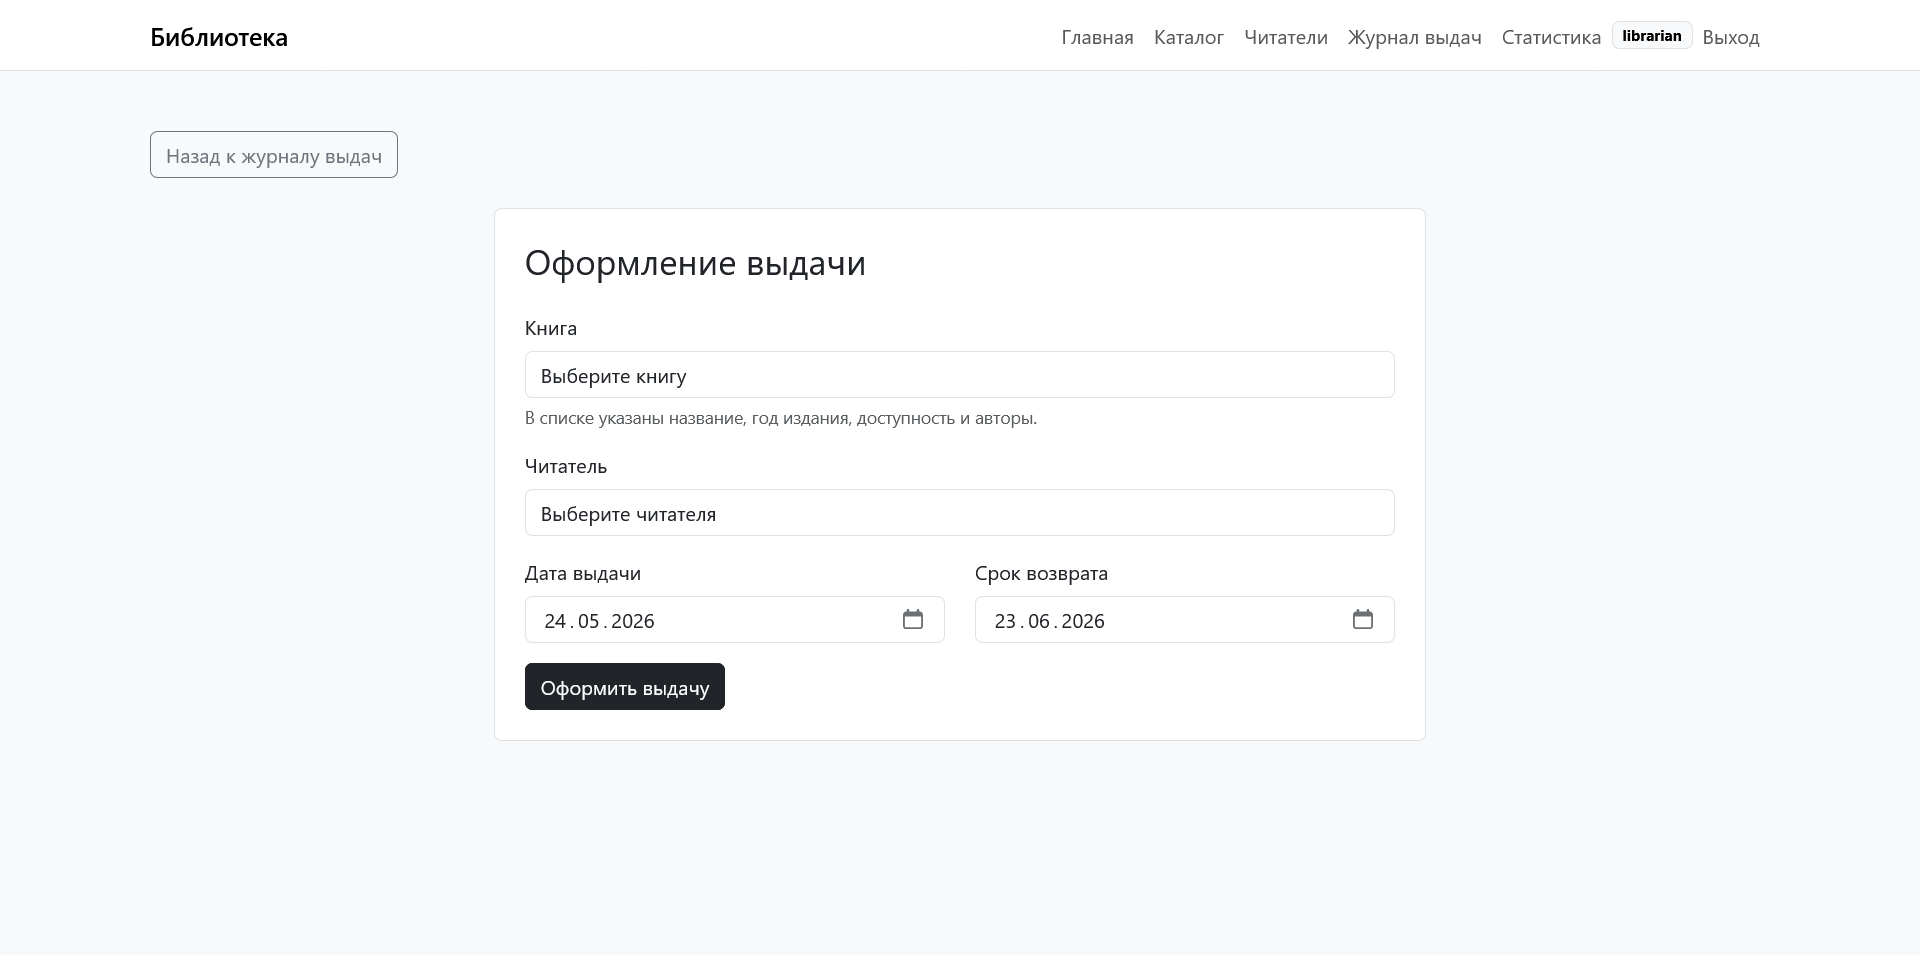
\includegraphics[width=0.85\textwidth]{images/app_loan_form.png}
\caption{Форма оформления выдачи книги}
\label{fig:app-loan-form}
\end{figure}

В форме выдачи отображаются только книги, у которых есть доступные экземпляры. При сохранении выдачи количество доступных экземпляров книги уменьшается на единицу. При возврате книги статус выдачи меняется на «возвращена», фиксируется дата возврата, а количество доступных экземпляров увеличивается.

Для защиты от некорректного ввода дат реализована проверка: срок возврата не может быть раньше даты выдачи, а фактическая дата возврата не может быть раньше даты выдачи.

\subsection{Реализация журнала выдач}

Журнал выдач предназначен для контроля всех операций выдачи и возврата книг. В журнале отображаются обложка, книга, читатель, дата выдачи, срок возврата, дата возврата, статус и доступные действия.

Страница журнала выдач представлена на рисунке~\ref{fig:app-loans}.

\begin{figure}[htbp]
\centering
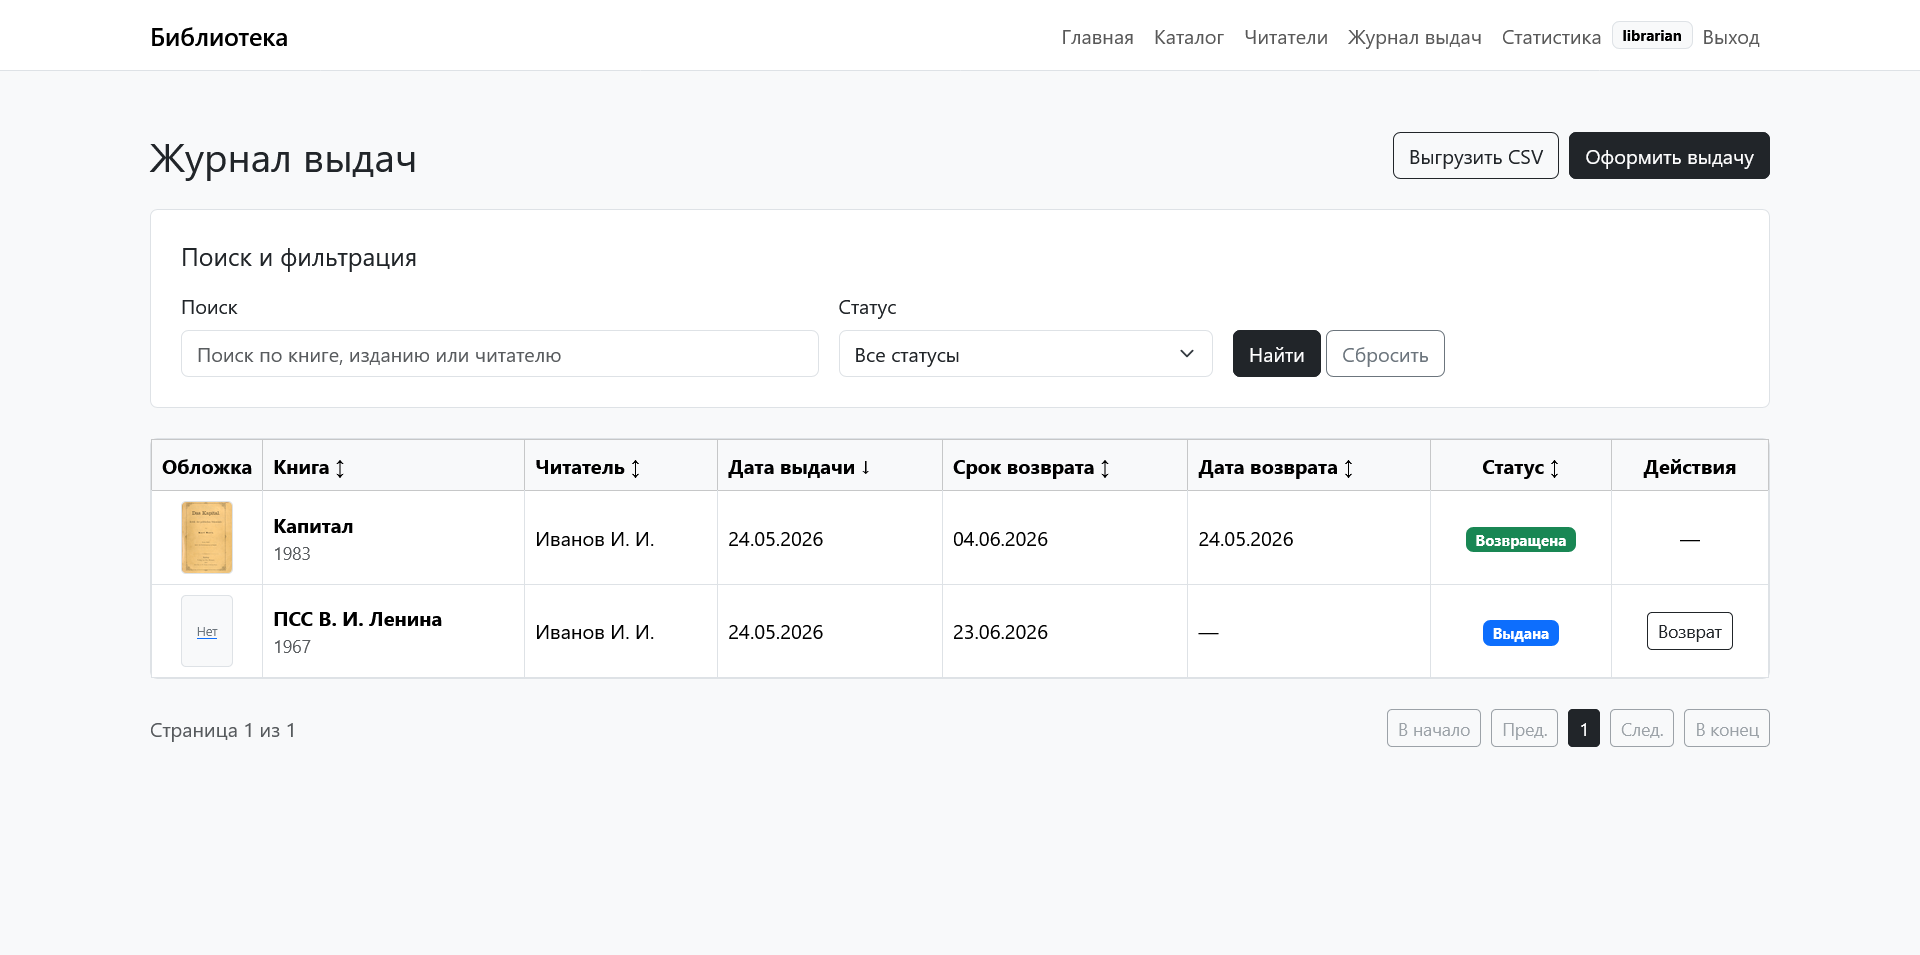
\includegraphics[width=0.95\textwidth]{images/app_loans.png}
\caption{Журнал выдач}
\label{fig:app-loans}
\end{figure}

В журнале реализованы:

\begin{itemize}
    \item поиск по книге, изданию или читателю;
    \item фильтрация по статусу;
    \item сортировка по основным столбцам;
    \item возврат книги;
    \item постраничная навигация;
    \item выгрузка журнала в CSV.
\end{itemize}

Просроченные выдачи автоматически обновляются при открытии страниц, связанных с выдачами и статистикой. Если срок возврата меньше текущей даты, а книга еще не возвращена, статус меняется на «просрочена».

\subsection{Реализация статистики}

Раздел статистики предназначен для анализа состояния библиотечного фонда и активности выдач. Пользователь может выбрать период отчета и категорию. По умолчанию период устанавливается с первого дня текущего месяца по текущую дату.

Страница статистики представлена на рисунке~\ref{fig:app-statistics}.

\begin{figure}[htbp]
\centering
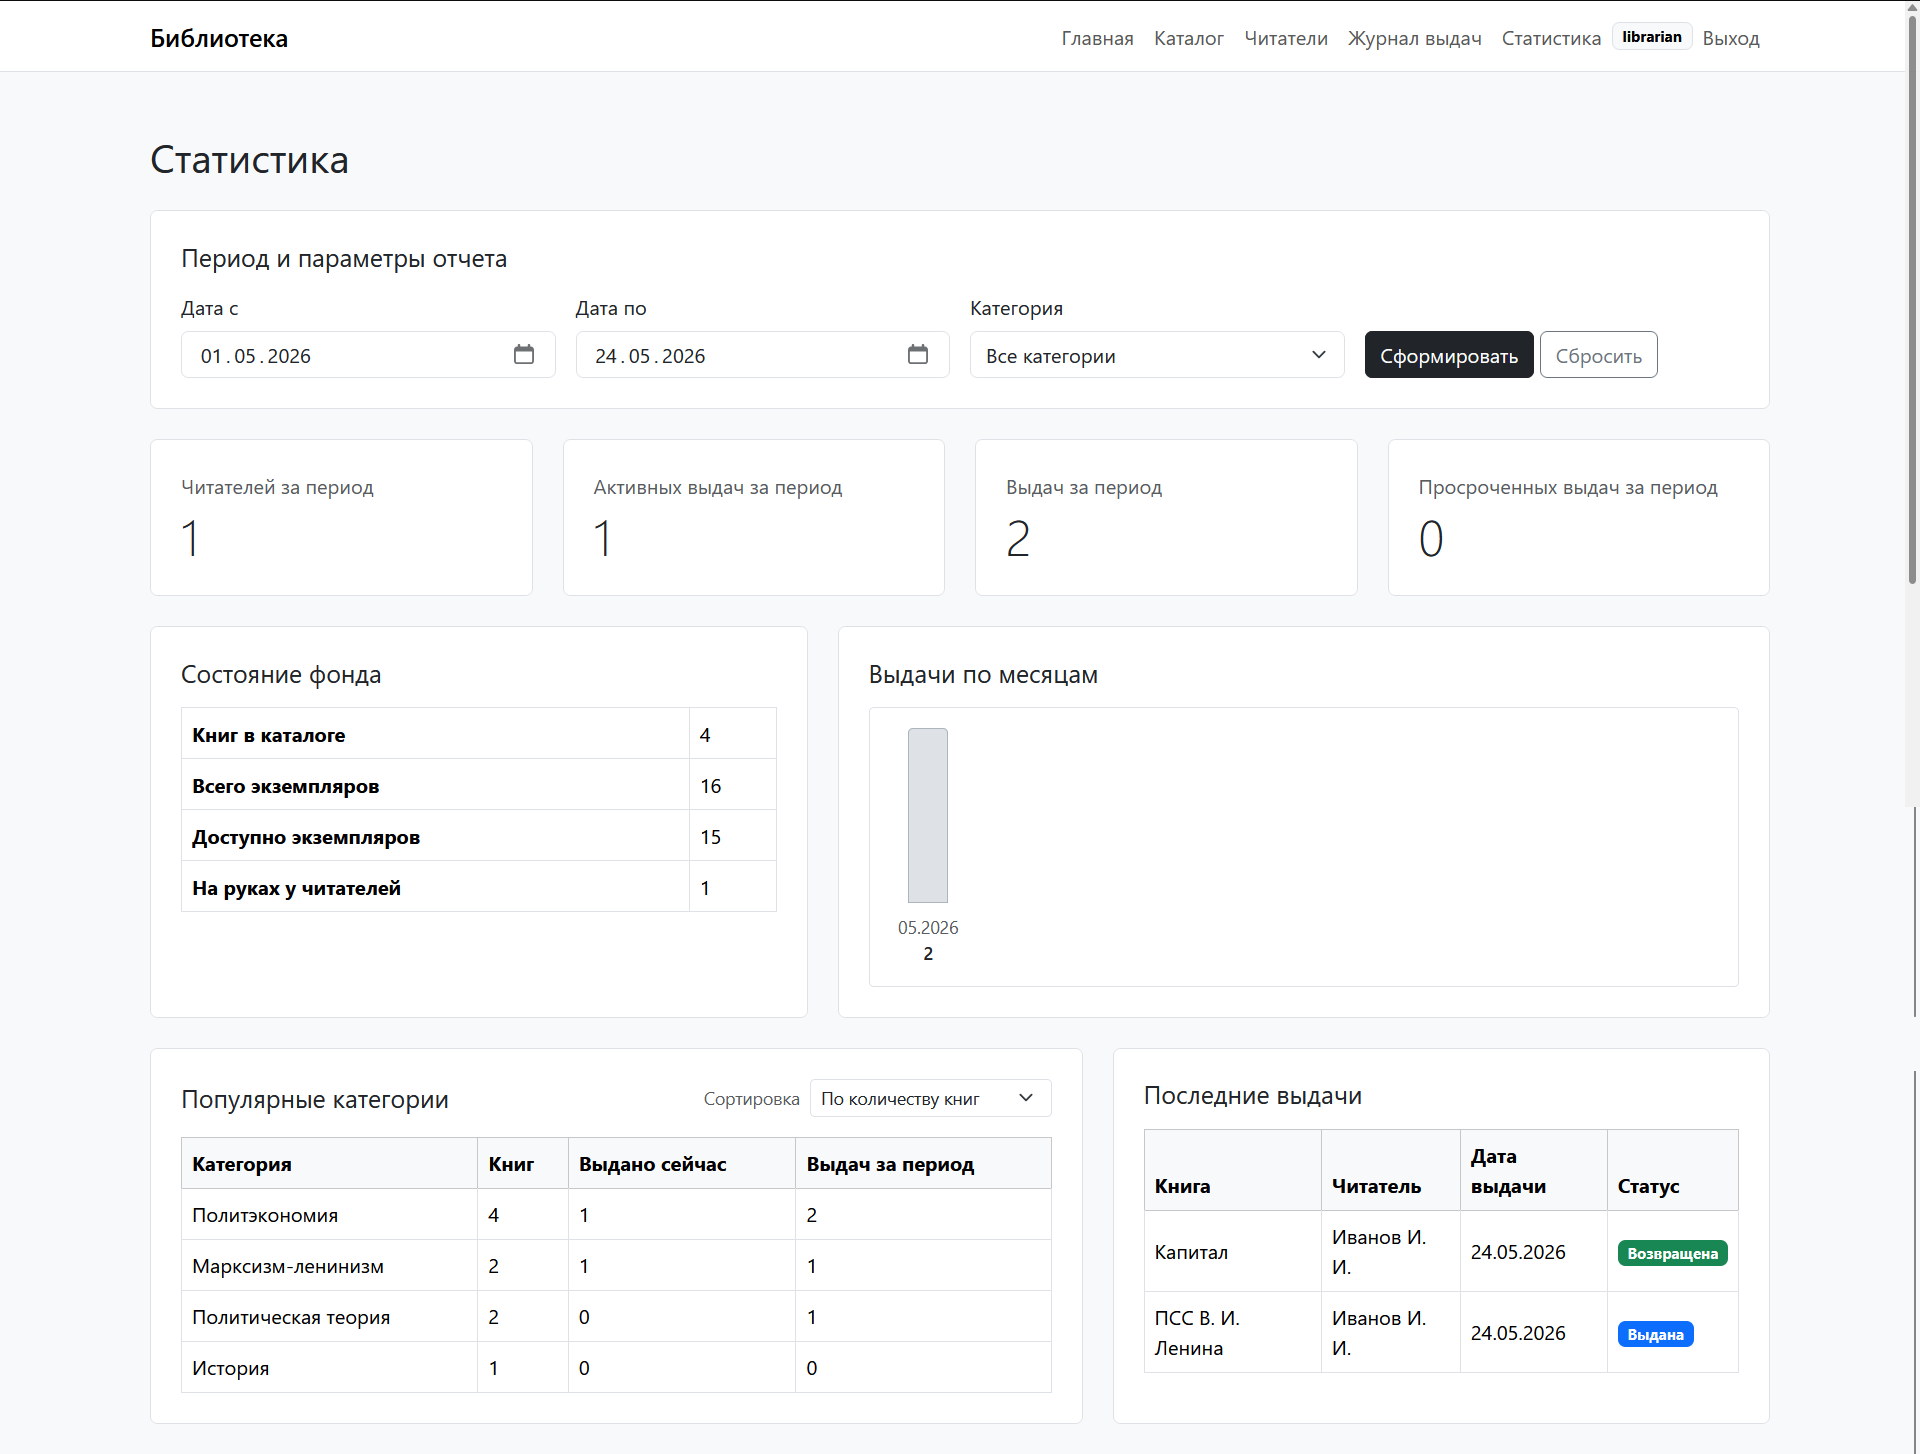
\includegraphics[width=0.95\textwidth]{images/app_statistics.png}
\caption{Страница статистики}
\label{fig:app-statistics}
\end{figure}

В статистике отображаются:

\begin{itemize}
    \item количество читателей, у которых в выбранный период была на руках хотя бы одна книга;
    \item количество активных выдач за период;
    \item количество выдач за период;
    \item количество просроченных выдач за период;
    \item состояние фонда;
    \item график выдач по месяцам;
    \item популярные категории;
    \item последние выдачи.
\end{itemize}

График выдач по месяцам строится на основе записей журнала выдач. Для группировки данных по месяцам используется функция \texttt{TruncMonth}. Популярные категории рассчитываются по количеству книг, количеству текущих выдач и количеству выдач за выбранный период.

\subsection{Реализация загрузки обложек и выгрузки CSV}

Загрузка файлов в приложении реализована на примере загрузки обложек книг. Обложка загружается через форму добавления или редактирования книги и сохраняется в каталоге \texttt{media/covers/}. В базе данных хранится путь к файлу.

Выгрузка данных реализована в формате CSV. Библиотекарь может выгрузить:

\begin{itemize}
    \item каталог книг;
    \item журнал выдач.
\end{itemize}

CSV-файл формируется сервером в момент запроса и сразу передается пользователю для скачивания. Для корректного открытия в табличных редакторах используется кодировка UTF-8 с BOM и разделитель «точка с запятой».

\subsection{Проверка работы приложения}

После реализации основных функций была выполнена ручная проверка работы приложения. Проверялись сценарии для разных ролей пользователей.

Для читателя проверялись:

\begin{itemize}
    \item регистрация;
    \item вход в систему;
    \item просмотр каталога;
    \item просмотр карточки книги;
    \item отсутствие доступа к журналу выдач, статистике и управлению книгами.
\end{itemize}

Для библиотекаря проверялись:

\begin{itemize}
    \item добавление книги;
    \item редактирование книги;
    \item загрузка обложки;
    \item удаление книги без истории выдач;
    \item оформление выдачи;
    \item возврат книги;
    \item просмотр журнала выдач;
    \item поиск, фильтрация и сортировка;
    \item просмотр статистики;
    \item выгрузка CSV;
    \item просмотр и редактирование данных читателей.
\end{itemize}

Для администратора проверялись:

\begin{itemize}
    \item вход в административную панель;
    \item управление пользователями;
    \item управление группами;
    \item назначение пользователям ролей.
\end{itemize}

В результате проверки основные функции приложения работают корректно. Реализованное приложение соответствует требованиям к курсовому проекту: оно поддерживает авторизацию, разграничение прав, работу с книгами, читателями, выдачами, статистикой, загрузку обложек и выгрузку данных.

Весь проект загружен на публичный Github репозиторий по адресу \url{https://github.com/Mark-Lender-241-3211/KP_WebDev_4sem}.